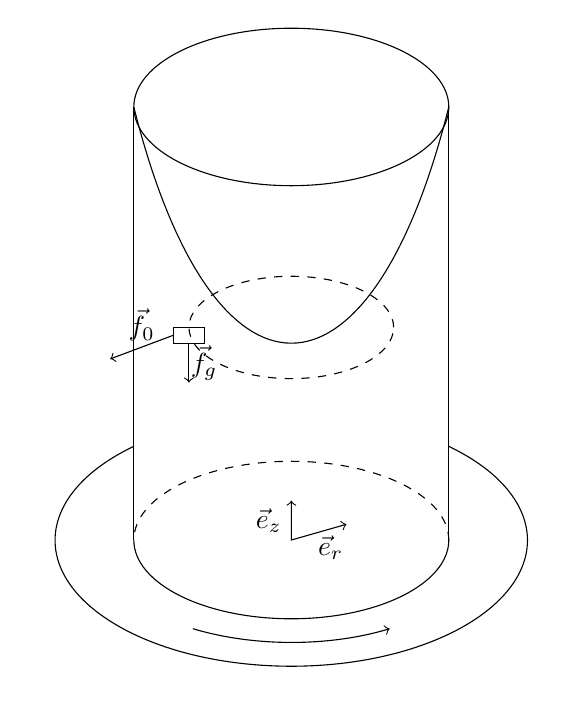
\begin{tikzpicture}
    \draw (-2, 2) coordinate (A) .. controls (-1, -2) and (1, -2) .. (2, 2) coordinate (B);
    \draw (A) -- (-2, -3.5);
    \draw (B) -- (2, -3.5);
    \draw (0, 2) ellipse (2 and 1);
    \draw[dashed] (0, -0.8) ellipse (1.3 and .65);
    \draw[dashed] (2, -3.5) arc (0:180:2 and 1);
    \draw         (-2, -3.5) arc (180:360:2 and 1);
    \draw         (-2, -2.31) arc (131.8:408.2:3 and 1.6);
    \draw[<->] (0, -3) -- (0, -3.5) -- (.7, -3.3);
    \node[left] at (0, -3.25) {$\vec e_z$};
    \node at (0.5, -3.6) {$\vec e_r$};
    \draw[->] (0, -3.5)+(240:2.5 and 1.3) arc (240:300:2.5 and 1.3);

    \draw (-1.5, -1) rectangle +(.4,.2);
    \draw[->] (-1.3, -1) -- +(0,-0.5);
    \node[right] at (-1.4, -1.25) {$\vec f_g$};
    \draw[->] (-1.5, -0.9) -- +(-0.8, -0.3);
    \node[above] at (-1.9, -1.1) {$\vec f_0$};
\end{tikzpicture}

